\section{シミュレーテッド・アニーリング}

\begin{frame}[t,fragile]{確率過程を用いた最適化}
  \begin{itemize}
    \setlength{\itemsep}{1em}
  \item 最急降下法 (steepest decent) {\footnotesize \href{https://github.com/todo-group/computer-experiments/blob/master/exercise/optimization/mc_steepest_descent_1d.c}{example-2-L4/mc\_steepest\_descent\_1d.c}}
    \begin{itemize}
    \item 初期状態をランダムに定める
    \item 配位を少しだけ変化させる
    \item エネルギー(コスト関数)が小さくなるなら採択、大きくなるなら棄却
    \item 状態が変化しなくなるまでくり返す %$\Rightarrow$ 絶対零度でのMetropolis法
    \item 問題点 : エネルギー極小状態にすぐに捕まってしまう
    \end{itemize}
  \item 徐冷法 (simulated annealing) {\footnotesize \href{https://github.com/todo-group/computer-experiments/blob/master/exercise/optimization/simulated_annealing_1d.c}{example-2-L4/simulated\_annealing\_1d.c}}
    \begin{itemize}
    \item いきなり温度を零にするのではなく少しずつ下げていく
    \item どれくらいゆっくり下げれば良いか? $
      T(t) \ge cN / \log(t+2)
      $
    \item 実際には適当なスケジューリングで温度を下げ、何回か繰り返して最も良い結果を採択
    \end{itemize}
  \end{itemize}
\end{frame}

\begin{frame}[t,fragile]{最急降下法とシミュレーテッド・アニーリング}
  \noindent\resizebox{0.45\textwidth}{!}{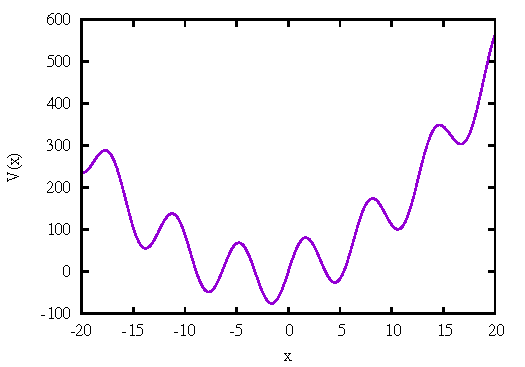
\includegraphics{image/potential.pdf}}

  \noindent\hspace*{.5em}\resizebox{0.43\textwidth}{!}{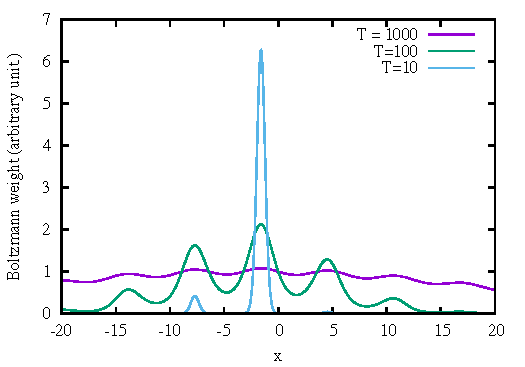
\includegraphics{image/boltzmann.pdf}}

  \vspace*{-17em}\hspace*{12.5em}\resizebox{0.6\textwidth}{!}{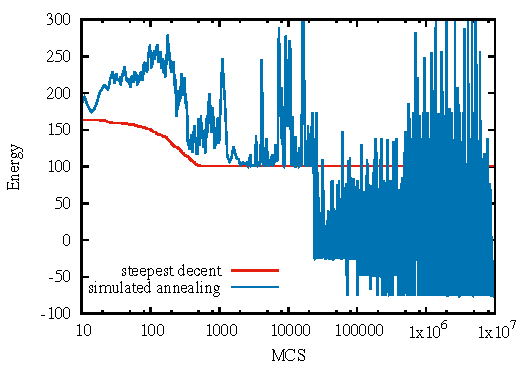
\includegraphics{image/energy.pdf}}

  \hspace*{17em}$T(t) = 100 - \frac{99}{10^7} t$
\end{frame}

\begin{frame}[t,fragile]{離散最適化問題への応用}
  \begin{itemize}
    \setlength{\itemsep}{1em}
  \item 微分を必要としないので、離散最適化問題にも適用可
    \begin{itemize}
    \item 例: 巡回セールスマン問題、数独、ナップザック問題
    \end{itemize}
  \item いかに状態とエネルギーを定義するかが重要
    \begin{itemize}
    \item 例: $n \times n$魔法陣 (行・列・ななめの和$M = n(n^2+1)/2$)
    \item 「状態」C: $1\sim n^2$の自然数をある順序でます目に並べたもの
    \item 「エネルギー」
      \[
      E(C) = \sum_{\rm row} (S_r-M)^2 + \sum_{\rm col} (S_c-M)^2 + \sum_{\rm diag} (S_d-M)^2
      \]
    \item 「正しい」魔方陣: $E(C) = 0$
    \end{itemize}
  \item 解の数(絶対零度のエントロピー)を求めるのにも利用できる
  \end{itemize}
\end{frame}
